\documentclass{standalone}
\usepackage{tikz}
\usepackage{ctex,siunitx}
\setCJKmainfont{Noto Serif CJK SC}
\usepackage{tkz-euclide}
\usepackage{amsmath}
\usetikzlibrary{patterns, calc,3d}
\usetikzlibrary{decorations.pathmorphing,decorations.pathreplacing,decorations.shapes}
\begin{document}
\small
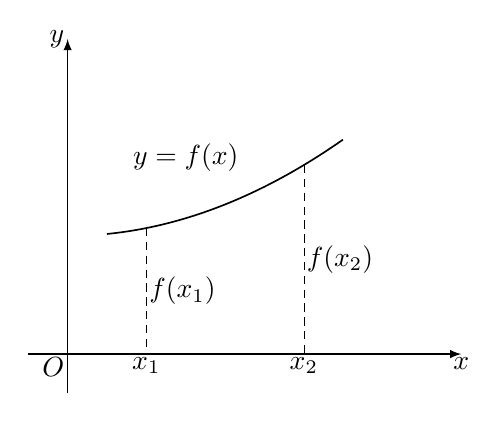
\begin{tikzpicture}[>=latex,scale=1.0,inner sep=1pt]
  \draw[->](-0.5,0)--(5,0)node[below]{$x$};
  \draw[->](0,-0.5)--(0,4)node[left]{$y$};
  \node at (0,0)[below left]{$O$};
  \draw[semithick,samples=200,domain=0.5:3.5]plot(\x,{1.5+0.1*\x*\x});
  \draw[very thin,densely dashed](1,1.6)--(1,0)node[below]{$x_1$}node[midway,right]{$f(x_1)$};
  \draw[very thin,densely dashed](3,2.4)--(3,0)node[below]{$x_2$}node[midway,right]{$f(x_2)$};
  \node at (1.5,2.5){$y=f(x)$};
\end{tikzpicture}
\end{document}